% Compilazione: pdflatex -jobname=elettrotecnica_tex elettrotecnica.tex
\documentclass[11pt,a4paper]{article}
\usepackage[utf8]{inputenc}\usepackage[T1]{fontenc}\IfFileExists{italian.ldf}{\usepackage[italian]{babel}}{\usepackage[english]{babel}}\usepackage{amsmath,amssymb,geometry,graphicx,circuitikz}\geometry{margin=22mm}
\newcommand{\pagina}[2]{\clearpage\section*{#2}}
\title{Elettrotecnica}\author{Trascrizione degli appunti}\date{}
\setlength{\emergencystretch}{3em}
\begin{document}\maketitle
% Pagina originale 1
\pagina{1}{Legenda}
\textbf{Corrente continua}: nozioni importanti; bipoli; generatori; bipoli reali e ideali; bipoli lineari; generatori dipendenti; cortocircuito e circuito aperto; resistenza; legge di Ohm; leggi di Kirchhoff; bipoli equivalenti; conduttanza; partitore di tensione; partitore di corrente; rendimento; passivazione; trasformazione generatori reali; semplificazioni ai generatori dipendenti; indicatori; resistenze stella--triangolo; teorema di Tellegen; PSE; prevalenza; teorema di Millman; teorema di Thevenin; teorema di Norton; massimo trasferimento di potenza; condensatore; induttore; circuiti del primo ordine (RC, RL); circuiti del secondo ordine (sovrasmorzamento, smorzamento critico, sottosmorzamento).

\textbf{Corrente alternata}: impedenza; triangolo delle impedenze; ammettenza; potenze; triangolo delle potenze; valore efficace; principio di conservazione della potenza; teorema di Boucherot; massimo trasferimento di potenza attiva; rifasamento (metodo delle potenze, metodo delle impedenze); risonanza RLC serie; risonanza RLC parallelo puro e non puro; campana di risonanza; frequenza di taglio; fattore di qualità; filtri; autoinduzione; mutua induzione; collegamento induttori accoppiati; energia di mutuo accoppiamento; leggi di Kirchhoff magnetiche; formule per nuclei ferromagnetici; trasformatore; trasformatore ideale; anti-trasformatore; trifase.
% Pagina originale 2
\pagina{2}{Nozioni importanti}
Principio di conservazione della carica: la carica elettrica non si può creare o distruggere, solo trasferire.
\[i=\frac{dq}{dt},\qquad j=\frac{di}{dS},\qquad \xrightarrow{x}\equiv\xleftarrow{-x}.\]
Esistono due tipi di corrente: stazionaria (regime stazionario), alternata (regime sinusoidale). La tensione è la differenza di potenziale. Anche la tensione può essere continua o alternata.
\[P=\frac{dw}{dt}=\frac{dw}{dq}\frac{dq}{dt}=Vi,\qquad [V\cdot A=W],\qquad 1\,W=\frac{1\,J}{1\,s}.\]
La potenza ha un segno e dipende dalla convenzione. Convenzione del generatore: $P<0$ assorbita, $P>0$ generata. Convenzione dell'utilizzatore: $P<0$ generata, $P>0$ assorbita.

Principio di conservazione dell'energia: la somma algebrica di tutte le potenze del circuito è nulla. Circuito elettrico a parametri concentrati (PC): è a PC se $\lambda_{\min}\gg D_{\max}$ ($\lambda_{\min}\geq10D_{\max}$), con $\lambda=c/f$ e $D$ dimensioni del circuito.
% Pagina originale 3
\pagina{3}{Bipoli e generatori}
Sono elementi circuitali con due morsetti (terminali). Bipoli attivi: generano potenza; passivi: consumano/assorbono potenza. Nota riportata: attivi non lineari, passivi lineari.

I generatori sono bipoli attivi. Possono essere indipendenti o dipendenti da parametri nel circuito.

I bipoli possono essere reali o ideali. Sono reali se hanno resistenza interna in serie e/o parallelo; ideali se perfetti senza alcuna resistenza interna.

I bipoli sono lineari se rappresentabili come una retta passante per l'origine prendendo due caratteristiche fisiche circuitali come assi. I generatori ideali non sono lineari, quelli reali sì. Caratteristica del generatore ideale di tensione: $V$ costante al variare di $I$. Generatore reale: $V=E-RI$; retta del resistore $V=RI$. La caratteristica del resistore è lineare.
% Pagina originale 4
\pagina{4}{Generatori dipendenti, resistenza}
Generatori di tensione/corrente controllati da tensione/corrente:
\[\begin{array}{c|c}GTCT&E=E_0v\\GTCC&E=R_0i\\GCCT&I=G_0v\quad[S=A/V]\\GCCC&I=I_0i\end{array}\]
Sono tutti bipoli lineari e passivi [come scritto nell'originale].

Cortocircuito: $V\to0$, $R\to0$. Circuito aperto: $I\to0$, $R\to\infty$. Tutto ciò che è in parallelo ad un cortocircuito o in serie ad un circuito aperto può essere eliminato.
\[R=\rho\frac{\ell}{A}\quad[\Omega].\]
Il resistore ha la caratteristica di opporsi al passaggio della corrente. Legge di Ohm:
\[R=\frac VI,\qquad V=RI.\]
Deriva direttamente dalla proporzionalità lineare e diretta tra $V$ e $I$. Deriva dalla linearità del resistore.
% Pagina originale 5
\pagina{5}{Leggi di Kirchhoff}
Definizioni: un ramo è un bipolo. Un nodo è un punto di interconnessione di due o più bipoli. Una maglia è un percorso chiuso che si ottiene partendo da un nodo $A$ di partenza e tornando su di esso attraversando i nodi una sola volta. Una maglia è indipendente se contiene un ramo non contenuto in altre maglie. Un nodo è degenere se collega solo due rami.

Dati $b$ rami, $\ell$ maglie indipendenti e $n$ nodi, la legge fondamentale dei circuiti elettrici dice che
\[b=\ell+n-1.\]
LKC: per qualsiasi nodo la somma delle correnti entranti è uguale alla somma delle correnti uscenti. LKT: per qualsiasi maglia la somma delle tensioni è nulla.

Bipoli equivalenti. Serie: due bipoli sono in serie se attraversati dalla stessa corrente. Per LKC $i_1=i_2$, dunque $R_1$ ed $R_2$ sono in serie. Sono in serie se condividono un morsetto esclusivo, un nodo.
% Pagina originale 6
\pagina{6}{Bipoli equivalenti e conduttanza}
\[E-R_1i-R_2i=0\quad\text{per LKT},\qquad E=i(R_1+R_2)=iR_{eq},\qquad R_{eq}=\sum_iR_i.\]
Parallelo: due bipoli sono in parallelo se ai loro capi insiste la stessa tensione.
\[E=R_1i_1=R_2i_2,\qquad i_1=\frac E{R_1},\quad i_2=\frac E{R_2}.\]
\[i_{eq}=i_1+i_2=\frac E{R_1}+\frac E{R_2}=E\left(\frac1{R_1}+\frac1{R_2}\right)=\frac E{R_{eq}},\]
\[\frac1{R_{eq}}=\frac1{R_1}+\frac1{R_2},\qquad\frac1{R_{eq}}=\sum_i\frac1{R_i}.\]
Sono in parallelo se sono collegati tra la stessa coppia di nodi. Generatori di tensione in serie, con polarità alternate nell'esempio: $E_{eq}=E_1-E_2+E_3$. Generatori di corrente in parallelo, con $I_1,I_2$ concordi e $I_3$ opposto: $I_{eq}=I_1+I_2-I_3$.

Conduttanza: $G=1/R$. Per $R_1\parallel R_2\parallel R_3\parallel\cdots\parallel R_m$, $G_{eq}=\sum_iG_i$, $R_{eq}=G_{eq}^{-1}$.
% Pagina originale 7
\pagina{7}{Partitori, rendimento, passivazione}
Partitore di tensione: circuito con generatore $E$ e $R_1,R_2,R_3$ in serie.
\[E-R_1i-R_2i-R_3i=0,\quad i=\frac E{R_1+R_2+R_3},\quad V_1=R_1i=\frac{R_1}{R_1+R_2+R_3}E,\quad V_m=\frac{R_m}{\sum_iR_i}E.\]
Partitore di corrente: $R_1,R_2$ in parallelo al generatore $I$.
\[I_1+I_2=I,\quad R_1I_1=R_2I_2,\quad R_1I_1=R_2(I-I_1),\quad I_1(R_1+R_2)=R_2I,\]
\[I_1=\frac{R_2}{R_1+R_2}I,\qquad I_m=\frac{G_m}{\sum_iG_i}I.\]
Rendimento del generatore:
\[\eta=\frac{P_e}{P_g}=\frac{-V_{AB}I}{-EI}=1-\frac{R_iI}{E}.\]
$\eta=1$ nei generatori ideali dove $R_i=0$. Nei generatori reali di corrente $\eta=1$ per $R_i\to\infty$. Resistenza interna in parallelo al generatore di corrente, in serie al generatore di tensione. Passivazione: generatore di tensione sostituito con cortocircuito ($V=0$); generatore di corrente con circuito aperto ($I=0$).
% Pagina originale 8
\pagina{8}{Trasformazione dei generatori reali}
Un generatore di tensione $E$ con $R_i$ in serie è equivalente a un generatore di corrente $I$ con $R_i$ in parallelo, con $I=E/R_i$. Usando il procedimento inverso per tornare allo stato precedente: $E=IR_i$. Non è applicabile a generatori ideali.

Semplificazioni ai generatori dipendenti. GTCC controllato dalla propria corrente: $V=\alpha I_0$, $R=V/I=\alpha I_0/I_0=\alpha$, equivalente a $R=\alpha\,\Omega>0$. GCCT controllato dalla propria tensione: $I=\alpha V_{AB}$, $R=V/I=V_{AB}/(\alpha V_{AB})=\alpha^{-1}$, equivalente a $R=1/\alpha\,\Omega>0$.

Indicatori: amperometro ideale in serie equivale a un filo; voltmetro ideale in parallelo equivale a un circuito aperto.
% Pagina originale 9
\pagina{9}{Resistenze stella--triangolo}
I resistori sono a stella quando hanno un nodo in comune. Sono a triangolo quando hanno un nodo in comune a due a due. Nel ponte illustrato: $R_1$ tra $A,B$; $R_2$ tra $B,C$; $R_3$ tra $B,D$; $R_4$ tra $C,D$; $R_5$ tra $C,E$; $R_6$ tra $D,E$; generatore tra $A,E$. $R_1,R_2,R_3$ sono a stella (nodo $B$); $R_2,R_4,R_5$ e $R_3,R_4,R_6$ sono a stella (nodi $C,D$). $R_2,R_3,R_4$ sono a triangolo ($C,B,D$), $R_4,R_5,R_6$ a triangolo ($C,D,E$).

Trasformazione $\Delta\to Y$: la stella ha $R_1$ verso il morsetto 1, $R_2$ verso 3, $R_3$ verso 2/4; il triangolo ha $R_c$ tra 1,3; $R_b$ tra 1,2; $R_a$ tra 3,4.
\[R_{1,2}=R_1+R_3,\quad R_{1,3}=R_1+R_2,\quad R_{3,4}=R_2+R_3.\]
\[R_{1,2}=(R_a+R_c)\parallel R_b,\quad R_{1,3}=(R_b+R_a)\parallel R_c,\quad R_{3,4}=(R_b+R_c)\parallel R_a.\]
Uguagliando le resistenze equivalenti:
\begin{align}R_1+R_3&=\frac{(R_a+R_c)R_b}{R_a+R_b+R_c},\tag{1}\\R_1+R_2&=\frac{(R_a+R_b)R_c}{R_a+R_b+R_c},\tag{2}\\R_2+R_3&=\frac{(R_b+R_c)R_a}{R_a+R_b+R_c}.\tag{3}\end{align}
% Pagina originale 10
\pagina{10}{Derivazione stella--triangolo}
Per trovare solo $R_1$ faccio $(2)-(3)+(1)\to2R_1$. Ponendo $R=R_a+R_b+R_c$:
\begin{align*}2R_1&=\frac{(R_a+R_b)R_c}{R}-\frac{(R_b+R_c)R_a}{R}+\frac{(R_a+R_c)R_b}{R}\\&=\frac{R_aR_c+R_bR_c-R_bR_a-R_aR_c+R_aR_b+R_bR_c}{R}=2\frac{R_bR_c}{R_a+R_b+R_c}.\end{align*}
\[R_1=\frac{R_bR_c}{R_a+R_b+R_c},\quad R_2=\frac{R_aR_c}{R_a+R_b+R_c},\quad R_3=\frac{R_aR_b}{R_a+R_b+R_c}.\]
Regola $\Delta\to Y$: prodotto delle resistenze adiacenti diviso la somma delle resistenze del triangolo.
\begin{align*}R_1R_2+R_1R_3+R_2R_3&=\frac{R_aR_bR_c^2+R_aR_b^2R_c+R_a^2R_bR_c}{(R_a+R_b+R_c)^2}\\&=\frac{R_aR_bR_c(R_a+R_b+R_c)}{(R_a+R_b+R_c)^2}=\frac{R_aR_bR_c}{R_a+R_b+R_c}.\tag{4}\end{align*}
\[\frac{R_1R_2+R_1R_3+R_2R_3}{R_1}=R_2+R_3+\frac{R_2R_3}{R_1}=\frac{R_aR_bR_c}{R_a+R_b+R_c}\frac{R_a+R_b+R_c}{R_bR_c}=R_a.\]
\[R_a=R_2+R_3+\frac{R_2R_3}{R_1},\quad R_b=R_1+R_3+\frac{R_1R_3}{R_2},\quad R_c=R_1+R_2+\frac{R_1R_2}{R_3}.\]
Regola $Y\to\Delta$: somma delle resistenze adiacenti più il prodotto delle adiacenti diviso la resistenza opposta.
% Pagina originale 11
\pagina{11}{Tellegen, sovrapposizione, prevalenza}
Teorema di Tellegen: la somma delle potenze di ogni singolo ramo è nulla.

Principio di sovrapposizione degli effetti (PSE): consiste nello spegnere tutti i generatori indipendenti eccetto uno, calcolare l'effetto di ogni singola componente e infine sommare gli effetti. Vale solo per caratteristiche lineari.
\[P=RI^2\ne R(I'^2+I''^2).\]
Prevalenza. In una maglia con generatore di tensione, resistore e generatore di corrente in serie, il PSE dà $I_R'=I_g$, $I_R''=0$, quindi $I=I_g$. Il generatore di corrente ha prevalenza con tutte le componenti in serie. In parallelo tra generatore di tensione, generatore di corrente e resistore: $I_R'=0$, $I_R''=E/R$, dunque $I_R=E/R$. Il generatore di tensione ha prevalenza con tutti i bipoli in parallelo. Due generatori di tensione diversi in parallelo costituiscono un assurdo fisico: passivandone uno si imporrebbe $0\,V$ sull'altro.
% Pagina originale 12
\pagina{12}{Millman}
Due generatori di corrente diversi in serie sono un assurdo fisico. Con il PSE si dimostra sia la prevalenza sia gli assurdi fisici: spegnendone uno si impone $I=0$ all'altro.

Teorema di Millman. Rami in parallelo: generatore di tensione $V_{Ai}$ in serie con $R_{Ai}$, generatore di corrente $I_{bj}$ in serie con $R_{bj}$, resistore $R_{ck}$.
\[I_0=\frac{V_{Ai}}{R_{Ai}}+I_{bj},\qquad R_0=\frac1{1/R_{Ai}+1/R_{ck}},\qquad V_0=R_0I_0.\]
Dimostrazione: trasformo il generatore di tensione in uno di corrente. Il resistore in serie al generatore di corrente è eliminato per prevalenza. Con $I_{Ai}=E_{Ai}/R_{Ai}$ sommo i generatori di corrente in parallelo e trovo la resistenza equivalente:
\[I_0=I_{Ai}+I_{bj}=\frac{E_{Ai}}{R_{Ai}}+I_{bj},\quad R_0=\frac1{1/R_{ck}+1/R_{Ai}},\quad V_0=I_0R_0.\]
Il circuito finale si trasforma in generatore $V_0$ con $R_0$ in serie tra $B,A$.
% Pagina originale 13
\pagina{13}{Thevenin}
Requisiti della rete: comunque complessa; tempo-invariante; lineare; univoca; nessun legame con grandezze elettriche esterne alla rete; accessibile da due morsetti.

Esempio: ramo sinistro $E_1,R_1$; $R_2$ collega il ramo sinistro al nodo $C$; dal nodo $C$ al riferimento $B$ sono in serie generatore di corrente $I$ (verso il basso) e $R_3$; $R_4$ tra $C,A$; $R_5,R_6$ tra $A,B$. Stacco $R_6$, elimino $R_3$ per prevalenza e applico Millman alla rete tra $C,B$, ottenendo $E_m,R_m$. Il circuito diventa $E_m,R_m,R_4,R_5$ in serie.
\[V_{AB}=\frac{R_5}{R_m+R_4+R_5}E_m=E_{Th}.\]
Passivo ogni generatore:
\[R_{Th}=\frac{(R_4+R_m)R_5}{R_4+R_m+R_5}.\]
% Pagina originale 14
\pagina{14}{Dimostrazione di Thevenin e Norton}
Dimostrazione di Thevenin: rete $N$ (black box) ai morsetti $A,B$. Applico un generatore di corrente tra $A,B$ e uso il PSE. Primo circuito: generatore esterno spento, $V'_{AB}=V_{AB0}$. Secondo: rete passivata $N_0$, $V''_{AB}=R_{eq}I$.
\[V_{AB}=V'_{AB}+V''_{AB}=V_{Th}+R_{Th}I.\]
Teorema di Norton: stesse ipotesi del teorema di Thevenin. Rete $N$ equivalente a $I_N$ in parallelo a $R_N$. Dimostrazione: applico un generatore di tensione $E$ e uso il PSE. Prima rete con generatore esterno cortocircuitato:
\[I'=I_{cc}=I_N.\]
Seconda rete passivata:
\[I''=-\frac E{R_{eq}},\qquad R_{eq}=R_N.\]
\[I=I'+I''=I_N-\frac E{R_N}.\]
% Pagina originale 15
\pagina{15}{Massimo trasferimento di potenza, condensatore}
Generatore equivalente $V_{Th}$ con $R_{Th}$ in serie al carico $R_L$:
\[P=R_LI^2,\qquad I=\frac{V_{Th}}{R_{Th}+R_L}.\]
Se $R_L=0$, $P\to0$; se $R_L\to\infty$, $P_L\to0$.
\[P=R_L\frac{V_{Th}^2}{(R_{Th}+R_L)^2}.\]
\begin{align*}\frac{\partial P}{\partial R_L}&=\frac{V_{Th}^2(R_{Th}+R_L)^2-R_LV_{Th}^2(2R_{Th}+2R_L)}{(R_{Th}+R_L)^4}\\&=\frac{(R_{Th}^2-R_L^2)V_{Th}^2}{(R_{Th}+R_L)^4}=\frac{(R_{Th}-R_L)V_{Th}^2}{(R_{Th}+R_L)^3}=0\end{align*}
$\Leftrightarrow R_{Th}=R_L$ (condizione di massimo trasferimento). $\eta=0.5$ quando $R_L/R_{Th}=1$.

Condensatore: bipolo passivo conservativo con la capacità di trattenere le cariche. La carica del condensatore misura quante cariche vengono separate, stessa differenza tra le due facce.
\[q=CV,\qquad[C=F\cdot V],\qquad[F=C/V],\]
\[\frac{dq}{dt}=i=\frac d{dt}(CV)\quad\Longrightarrow\quad i=C\frac{dV}{dt}.\]
Relazione lineare. In corrente continua ($dV/dt=0$) il condensatore equivale a circuito aperto.
% Pagina originale 16
\pagina{16}{Energia del condensatore, induttore}
\[P=Vi=VC\frac{dV}{dt},\quad W=\int_{-\infty}^tP\,dt=\int_{-\infty}^tCV\frac{dV}{dt}dt=\int_0^{V(t)}CV\,dV=\frac12CV^2.\]
\[W=\int_t^\infty P\,dt=\int_t^\infty CV\frac{dV}{dt}dt=\int_{V(t)}^0CV\,dV=-\frac12CV^2.\]
Condensatori in parallelo: $i_{eq}=i_1+i_2+i_3$, con $i_k=C_kdV/dt$ e $dV/dt$ uguale.
\[i_{eq}=(C_1+C_2+C_3)\frac{dV}{dt}=C_{eq}\frac{dV}{dt},\quad C_{eq}=\sum_iC_i.\]
Serie: $i_{eq}=C_1dV_1/dt=C_2dV_2/dt=C_3dV_3/dt$.
\[V=\frac1{C_1}\int i\,dt+\frac1{C_2}\int i\,dt+\frac1{C_3}\int i\,dt+\sum_{i=1}^3V_i(t_0),\]
\[V=\left(\frac1{C_1}+\frac1{C_2}+\frac1{C_3}\right)\int i\,dt+V_{eq}(t_0),\quad \frac1{C_{eq}}=\sum_i\frac1{C_i},\quad V_{eq}(t_0)=\sum_iV_i(t_0).\]
Induttore: bipolo passivo conservativo costituito da un filo conduttore avvolto in più spire. Conserva energia all'interno del proprio campo magnetico.
\[V=L\frac{di}{dt},\qquad L=\frac{N^2}{\mathcal R},\]
$N$ numero di spire, $\mathcal R$ riluttanza. Unità annotate $[H=A/m]$ [così nell'originale]. Relazione lineare; in corrente continua ($di/dt=0$) equivale a cortocircuito.
% Pagina originale 17
\pagina{17}{Induttori equivalenti}
\[V=L\frac{di}{dt}\Rightarrow i=\frac1L\int_{-\infty}^tV\,dt=\frac1L\int_{t_0}^tV\,dt+i(t_0),\quad P=Vi=L\frac{di}{dt}i.\]
\[W=\int_{-\infty}^tP\,dt=\int_{-\infty}^tLi\frac{di}{dt}dt=\int_0^{i(t)}Li\,di=\frac12Li^2,\quad \int_t^\infty P\,dt=-\frac12Li^2.\]
Serie: $V_1=L_1di/dt$, $V_2=L_2di/dt$, $V_3=L_3di/dt$;
\[V_{eq}=(L_1+L_2+L_3)\frac{di}{dt}=L_{eq}\frac{di}{dt},\quad L_{eq}=\sum_iL_i.\]
Parallelo:
\[V=L_1\frac{di_1}{dt}=L_2\frac{di_2}{dt}=L_3\frac{di_3}{dt},\]
\[i=\frac1{L_1}\int_{t_0}^tVdt+\frac1{L_2}\int_{t_0}^tVdt+\frac1{L_3}\int_{t_0}^tVdt+i_1(t_0)+i_2(t_0)+i_3(t_0),\]
\[i=\frac1{L_{eq}}\int_{t_0}^tVdt+i_{eq}(t_0),\qquad\frac1{L_{eq}}=\sum_i\frac1{L_i}.\]
% Pagina originale 18
\pagina{18}{Circuiti del primo ordine: RC naturale}
L'ordine del circuito è dato dal numero di bipoli reattivi (RL e RC). Per risolvere un circuito di ordine $n$ bisogna risolvere un'equazione differenziale di ordine $n$. Due tipi di risposta: libera/naturale e forzata; risposta completa = libera + forzata.

Circuito RC, risposta naturale (nessun generatore indipendente): resistore e condensatore collegati chiudendo l'interruttore $T$ a $t=0$.
\[i_C=C\frac{dV}{dt},\quad V_C=\frac1C\int i\,dt,\quad \frac VR+C\frac{dV}{dt}=0\Rightarrow\frac{dV}{V}+\frac{dt}{RC}=0.\]
\[\int_{V_0}^{V(t)}\frac{dV}{V}=-\int_0^t\frac1{RC}dt\Rightarrow\log\frac{V(t)}{V_0}=-\frac t{RC},\]
\[V(t)=V_0e^{-t/(RC)}=V_0e^{-t/\tau},\quad\tau=RC.\]
\[V(\tau)=0.368V_0,\quad V(2\tau)=0.135V_0,\quad V(5\tau)=0.00674V_0.\]
\[W_C(t)=\frac12CV_0^2e^{-2t/\tau},\quad W_R=\int_0^tP_Rdt=\int_0^t\frac{V_0^2}{R}e^{-2t/\tau}dt=\frac12CV_0^2(1-e^{-2t/\tau}).\]
% Pagina originale 19
\pagina{19}{RC: risposta forzata e completa}
\[W=W_C+W_R=\frac12CV_0^2,\quad W_C=\frac12CV_0^2e^{-2t/\tau},\quad W_R=\frac12CV_0^2(1-e^{-2t/\tau}).\]
Risposta forzata (condizioni iniziali nulle, $V_0=0$): generatore $V_s$, resistore $R$, condensatore $C$ in serie.
\[i_C=C\frac{dV}{dt},\quad V_C=\frac1C\int i\,dt,\quad V_{AB}=V_s+Ri_R\Rightarrow i_R=\frac{V_{AB}-V_s}{R}.\]
\[\frac{V_{AB}-V_s}{R}+C\frac{dV}{dt}=0\quad(i_R+i_C=0),\quad\frac{dV}{V_{AB}-V_s}=-\frac{dt}{RC},\]
\[\int_{V_0}^{V(t)}\frac{dV}{V-V_s}=-\int_0^t\frac{dt}{RC}\Rightarrow\log\frac{V(t)-V_s}{V_0-V_s}=-\frac t{RC}.\]
\[V(t)=V_s+(V_0-V_s)e^{-t/\tau}.\]
Con $V_0=0$: $V_F(t)=V_s-V_se^{-t/\tau}$. Risposta completa:
\[V_N(t)=V_0e^{-t/\tau},\quad V_F(t)=V_s-V_se^{-t/\tau},\quad V(t)=V_F(t)+V_N(t)=V_s+(V_0-V_s)e^{-t/\tau}.\]
Grafici: se $V_0>V_s$ la risposta completa decresce da $V_0$ a $V_s$; se $V_0<V_s$ cresce da $V_0$ a $V_s$; naturale decade a zero, forzata cresce da zero a $V_s$.
% Pagina originale 20
\pagina{20}{Circuito RL}
Risposta naturale (nessun generatore indipendente):
\[V_L=L\frac{di}{dt},\quad i_L=\frac1L\int V_Ldt,\quad V_R+V_L=0\Rightarrow Ri+L\frac{di}{dt}=0.\]
\[\frac{di}{i}=-\frac RLdt,\quad\int_{i_0}^{i(t)}\frac{di}{i}=-\int_0^t\frac RLdt\Rightarrow\log\frac{i(t)}{i_0}=-\frac RLt,\]
\[i_N(t)=i_0e^{-t/\tau},\qquad\tau=L/R.\]
\[W_L=\frac12Li^2=\frac12Li_0^2e^{-2t/\tau},\quad W_R=\int_0^tPdt=\int_0^tRi_0^2e^{-2t/\tau}dt=\frac12Li_0^2(1-e^{-2t/\tau}),\]
\[W=W_L+W_R=\frac12Li_0^2.\]
Risposta forzata: generatore $V_s$, $R,L$ in serie.
\[V_R+V_L-V_s=0,\quad Ri+L\frac{di}{dt}-V_s=0\Rightarrow\frac LR\frac{di}{dt}+i-\frac{V_s}{R}=0,\]
\[\frac{di}{i-V_s/R}=-\frac RLdt,\quad\int_{i_0=0}^{i(t)}\frac{di}{i-V_s/R}=-\int_0^t\frac RLdt,\]
\[\log\frac{i(t)-V_s/R}{i_0-V_s/R}=-\frac RLt\Rightarrow i_F(t)=\frac{V_s}{R}-\frac{V_s}{R}e^{-t/\tau},\quad\tau=L/R.\]
% Pagina originale 21
\pagina{21}{RL completo e circuiti del secondo ordine}
\[i_N(t)=i_0e^{-t/\tau},\quad i_F(t)=\frac{V_s}{R}(1-e^{-t/\tau})\Rightarrow i(t)=\frac{V_s}{R}+\left(i_0-\frac{V_s}{R}\right)e^{-t/\tau}.\]
Grafici della risposta: se $i_0>V_s/R$ la completa decresce verso $V_s/R$; se $i_0<V_s/R$ cresce verso $V_s/R$. La naturale tende a zero e la forzata a $V_s/R$ (indicazione $5\tau$).
\[i(t)=i_\infty+(i_0-i_\infty)e^{-t/\tau}\quad(RL:\tau=L/R),\]
\[V(t)=V_\infty+(V_0-V_\infty)e^{-t/\tau}\quad(RC:\tau=RC).\]
Circuiti del secondo ordine, RLC serie (risposta naturale): $R,L,C$ in serie, $i(0)=i_0$, $V(0)=V_0$.
\[R\frac{di}{dt}+L\frac{d^2i}{dt^2}+\frac iC=0.\]
% Pagina originale 22
\pagina{22}{Smorzamento}
\[\alpha=\frac R{2L}\quad\text{smorzamento},\qquad\omega_0=\frac1{\sqrt{LC}}\quad\text{frequenza di oscillazione (risonanza)}.\]
Se $\alpha>\omega_0$, $s_1,s_2\in\mathbb R$: sovrasmorzamento. Se $\alpha=\omega_0$, $s_1=s_2\in\mathbb R$: smorzamento critico. Se $\alpha<\omega_0$, $s_1,s_2\in\mathbb C\setminus\mathbb R$: sottosmorzamento.
\[\text{Sovrasmorzamento:}\quad i=A_1e^{s_1t}+A_2e^{s_2t}.\]
\[\text{Smorzamento critico:}\quad i=(A_1t+A_2)e^{-\alpha t}.\]
\[\text{Sottosmorzamento:}\quad i=e^{-\alpha t}[B_1\cos(\omega_dt)+B_2\sin(\omega_dt)],\quad B_1=A_1+A_2,\quad B_2=j(A_1-A_2).\]
Grafici: sovrasmorzato e critico tendono a zero senza oscillazioni; sottosmorzato oscilla con inviluppo esponenziale decrescente per $R>0$, crescente e instabile per $R<0$.
% Pagina originale 23
\pagina{23}{Corrente alternata e fasori}
\[V(t)=V_{\max}\cos(\omega t+\varphi_v),\quad i(t)=I_{\max}\sin(\omega t+\varphi_i),\quad f=\frac1T,\quad\omega=2\pi f=\frac{2\pi}T.\]
In anticipo $\varphi>0$, in ritardo $\varphi<0$. Valori riportati negli appunti (conservati): in Italia $f=50\,Hz\Rightarrow\omega=314\,rad/s$, $V_{\max}=220\,V$, $V_{eff}=V_{\max}/\sqrt2=155.5\,V$. In USA $f=60\,Hz\Rightarrow\omega=377\,rad/s$, $V_{\max}=110\,V$, $V_{eff}=V_{\max}/\sqrt2=77.8\,V$.

Formule di Werner:
\[\sin\alpha\sin\beta=\tfrac12[\cos(\alpha-\beta)-\cos(\alpha+\beta)],\quad\cos\alpha\cos\beta=\tfrac12[\cos(\alpha-\beta)+\cos(\alpha+\beta)].\]
\[z=x+jy,\quad r=\sqrt{x^2+y^2},\quad\theta=\arctan(y/x),\quad z=r\angle\theta,\]
\[z_1z_2=r_1r_2\angle(\theta_1+\theta_2),\quad z_1/z_2=(r_1/r_2)\angle(\theta_1-\theta_2).\]
Il fasore è un vettore rotante immaginato ad un tempo $\bar t$: un numero complesso che descrive ampiezza e fase.
\[v(t)=V_m\cos(\omega t+\varphi_v)\Rightarrow\dot V=V_m\angle\varphi_v.\]
% Pagina originale 24
\pagina{24}{Impedenza}
\[\dot V_R=R\dot I\ (\varphi_v=\varphi_i),\quad \dot V_L=j\omega L\dot I\ (\varphi_v=\varphi_i+\pi/2),\quad\dot V_C=-\frac j{\omega C}\dot I\ (\varphi_v=\varphi_i-\pi/2).\]
\[-\dot E+R\dot I+j\omega L\dot I-\frac j{\omega C}\dot I=0\quad\text{LKT},\]
\[\dot E=\left(R+j\omega L-\frac j{\omega C}\right)\dot I,\quad\frac{\dot E}{\dot I}=R+j\left(\omega L-\frac1{\omega C}\right)=\bar Z\in\mathbb C.\]
\[\bar Z=R+jX,\quad X=\omega L-\frac1{\omega C}\in\mathbb R\quad\text{reattanza},\quad\bar Z=\bar Z_R+\bar Z_L+\bar Z_C,\]
\[\bar Z_R=R,\quad\bar Z_L=j\omega L,\quad\bar Z_C=-\frac j{\omega C},\quad X=X_L-X_C,\quad X_L=\omega L,\quad X_C=\frac1{\omega C}.\]
Triangolo delle impedenze: cateto orizzontale $R$, verticale $X$, ipotenusa $|\bar Z|=\sqrt{R^2+X^2}$ e angolo $\varphi$. $X_L>X_C\Rightarrow X>0$: RL, impedenza ohmico-induttiva; $X_L<X_C\Rightarrow X<0$: RC, ohmico-capacitiva. Triangoli degeneri: solo resistore lungo asse reale ($|Z|=R$), solo induttore verso l'alto ($|Z|=X_L$), solo condensatore verso il basso ($|Z|=X_C$).
% Pagina originale 25
\pagina{25}{Ammettenza e potenze}
Diagramma fasoriale: $\varphi''>0\Rightarrow X>0$ (RL), $\varphi'<0\Rightarrow X<0$ (RC).
\[\bar Y=\frac1{\bar Z}=\frac1{R+jX}=\frac{R-jX}{R^2+X^2}=\frac{R-jX}{|\bar Z|^2}=\frac{\bar Z^*}{|\bar Z|^2},\]
\[\bar Y=G+jB\quad(G:\text{conduttanza},\ B:\text{suscettanza}),\quad G=\frac R{R^2+X^2}.\]
Nell'originale $B=-jX/(R^2+X^2)$ [fattore $j$ conservato]. Potenze (segni come nell'originale):
\[p(t)=v(t)i(t)=\tfrac12V_mI_m\cos\Delta\varphi-\tfrac12V_mI_m\cos\Omega,\quad\Omega=2\omega t+\varphi,\quad\Delta\varphi=\varphi_v-\varphi_i,\quad\varphi=\varphi_v+\varphi_i.\]
Potenza fluttuante:
\[P_f(t)=-\tfrac12V_mI_m\cos(2\omega t+\varphi).\]
\[\cos(2\omega t+\varphi)=\cos2\omega t\cos\varphi-\sin2\omega t\sin\varphi,\]
\[p(t)=\tfrac12V_mI_m\cos\Delta\varphi-\tfrac12V_mI_m\cos2\omega t\cos\varphi+\tfrac12V_mI_m\sin2\omega t\sin\varphi.\]
Potenza attiva istantanea e reattiva istantanea:
\[P_A(t)=\tfrac12V_mI_m\cos\Delta\varphi-\tfrac12V_mI_m\cos2\omega t\cos\varphi,\quad P_R(t)=\tfrac12V_mI_m\sin2\omega t\sin\varphi.\]
\[P=\frac1T\int_0^Tp(t)dt=\langle p(t)\rangle=\tfrac12V_mI_m\cos\Delta\varphi,\quad Q=\tfrac12V_mI_m\sin\varphi=\max P_R(t).\]
% Pagina originale 26
\pagina{26}{Potenze, valore efficace}
Potenza apparente $S=\tfrac12I_mV_m=\max P_f(t)$. Complessa $P_c=P+jQ$, $|P_c|=S$. Fattore di potenza $f_{dp}=P/S=\cos\Delta\varphi$.

Ricapitolando:
\[p(t)=P+P_f(t)=P_A(t)+P_R(t),\quad P=\langle P_A(t)\rangle,\quad Q=\max P_R(t),\]
\[S=\max P_f(t)=|P_c|,\quad P_c=P+jQ,\quad f_{dp}=\cos\Delta\varphi=P/S.\]
$\Delta\varphi=\varphi$ perché $\varphi_i=0$, dunque $\varphi_v-\varphi_i=\varphi_v+\varphi_i$. Triangolo delle potenze: cateti $P,Q$, ipotenusa $|P_c|=S$, angolo $\varphi$; $Q>0$ verso l'alto, $Q<0$ verso il basso.

Valore efficace (root mean square):
\[I_{eff}=\sqrt{\frac1T\int_0^Ti^2dt}=\frac{I_m}{\sqrt2},\qquad V_{eff}=\frac{V_m}{\sqrt2}.\]
Principio di conservazione delle potenze:
\[\sum P=0,\quad\sum Q=0,\quad\sum P_c=0,\qquad\sum S\ne0.\]
Somma delle potenze attive, reattive e complesse nulla.
% Pagina originale 27
\pagina{27}{Boucherot e massimo trasferimento di potenza attiva}
\[P_T=P_1+P_2+P_3,\quad Q_T=Q_1+Q_2+Q_3,\quad S_T=\sqrt{P_T^2+Q_T^2}.\]
\[S_T=S_1+S_2+S_3\Leftrightarrow\varphi_1=\varphi_2=\varphi_3.\]
Se $\varphi_1\ne\varphi_2$, $S_T\ne S_1+S_2$.

Massimo trasferimento di potenza attiva: $Z_{Th}=R_{Th}+jX_{Th}$, $Z_L=R_L+jX_L$.
\[P=\tfrac12R_L|\dot I|^2,\quad\dot I=\frac{\dot V_{Th}}{(R_{Th}+R_L)+j(X_{Th}+X_L)}=\frac{\dot V_{Th}}{\bar Z_{Th}+\bar Z_L},\]
\[P=\tfrac12R_L\left(\frac{|\dot V_{Th}|}{\sqrt{(R_{Th}+R_L)^2+(X_{Th}+X_L)^2}}\right)^2.\]
\[\frac{\partial P}{\partial X_L}=-\tfrac12R_L\frac{|V_{Th}|^2\,2(X_{Th}+X_L)}{[(R_{Th}+R_L)^2+(X_{Th}+X_L)^2]^2}=0\Rightarrow X_{Th}=-X_L.\]
\[\frac{\partial P}{\partial R_L}=\tfrac12\frac{|V_{Th}|^2(R_{Th}+R_L)^2-2R_L|V_{Th}|^2(R_{Th}+R_L)}{(R_{Th}+R_L)^4}=0\Rightarrow R_{Th}=R_L.\]
\[R_{Th}=R_L\ \wedge\ X_{Th}=-X_L\Rightarrow\bar Z_{Th}=\bar Z_L^*.\]
% Pagina originale 28
\pagina{28}{Rifasamento}
Inserire un condensatore in serie o parallelo consente di cambiare la fase tra le componenti. In parallelo è possibile staccare e attaccare senza interrompere il circuito.

Metodo delle potenze: triangolo con $P$ invariata, reattiva iniziale $Q_1$, finale $Q_2$, angoli $\varphi_1,\varphi_2$.
\[Q_C=Q_1-Q_2=P(\tan\varphi_1-\tan\varphi_2),\quad Q_C=\frac{|V_{eff}|^2}{X_C}=\omega C|V_{eff}|^2,\]
\[C=\frac{P(\tan\varphi_1-\tan\varphi_2)}{\omega|V_{eff}|^2}.\]
Metodo delle impedenze: $\bar Z_L=R+j\omega L$, $\bar Z_C=-j/(\omega C)$ in parallelo.
\[\bar Z_{eq}=\frac{\bar Z_L\bar Z_C}{\bar Z_L+\bar Z_C}=\frac{-jR/(\omega C)+L/C}{R+j(\omega L-1/(\omega C))}.\]
\[\bar Z_{eq}=\frac{(-jR/(\omega C)+L/C)[R-j(\omega L-1/(\omega C))]}{R^2+(\omega L-1/(\omega C))^2}\]
\[=\frac{-jR^2/(\omega C)+LR/C-LR/C-j\omega L^2/C+R/(\omega^2C^2)+jL/(\omega C^2)}{R^2+(\omega L-1/(\omega C))^2}.\]
\[\tan\varphi_2=\frac{\Im\bar Z_{eq}}{\Re\bar Z_{eq}}=\frac{-R^2/(\omega C)-\omega L^2/C+L/(\omega C^2)}{R/(\omega^2C^2)}=\frac{\omega(L-R^2C-\omega^2L^2C)}R.\]
\[\tan\varphi_2=-\frac{\omega C}{R}(R^2+\omega^2L^2)+\frac{\omega L}R,\quad\tan\varphi_1=\frac{\omega L}R=\frac{X_L}{R_L}.\]
% Pagina originale 29
\pagina{29}{Risonanza serie e parallelo puro}
\[\tan\varphi_2-\tan\varphi_1=-\frac{\omega C}R|Z|^2\Rightarrow\tan\varphi_1-\tan\varphi_2=C\frac{\omega|Z|^2}R,\quad C=\frac{R(\tan\varphi_1-\tan\varphi_2)}{\omega|Z|^2}.\]
Si può usare solo se a destra e sinistra di $A,B$ non ci sono generatori indipendenti/dipendenti.

Risonanza RLC serie: $E,R,C,L$ in serie.
\[-\dot E+R\dot I+j\omega L\dot I-\frac j{\omega C}\dot I=0\Rightarrow\dot E=\dot I\left[R+j\left(\omega L-\frac1{\omega C}\right)\right].\]
Condizione di risonanza $\dot E=R\dot I$ ($\Delta\varphi=0$):
\[\omega L-\frac1{\omega C}=0\Rightarrow\omega=\frac1{\sqrt{LC}}\Rightarrow f_0=\frac\omega{2\pi}=\frac1{2\pi\sqrt{LC}}.\]
Risonanza RLC parallelo puro: generatore di corrente con $R,L,C$ in parallelo.
\[\bar Y_R=G=\frac1R,\quad\bar Y_L=\frac1{j\omega L}=-\frac j{\omega L},\quad\bar Y_C=j\omega C,\]
\[\bar Y_{tot}=\frac1R+j\left(\omega C-\frac1{\omega L}\right),\quad\omega C-\frac1{\omega L}=0\Rightarrow\omega=\frac1{\sqrt{LC}},\quad f_0=\frac1{2\pi\sqrt{LC}}.\]
$B=0$ (annotazione originale $B=X^{-1}$).
% Pagina originale 30
\pagina{30}{Risonanza parallelo non puro}
Due rami in parallelo: $R_L,L$ in serie e $R_C,C$ in serie.
\[\bar Z_L=R_L+j\omega L,\quad\bar Z_C=R_C-\frac j{\omega C},\]
\[\bar Y_{tot}=\frac1{R_L+jX_L}+\frac1{R_C-jX_C}=\frac{R_L-jX_L}{R_L^2+X_L^2}+\frac{R_C+jX_C}{R_C^2+X_C^2}.\]
\[\Im\bar Y_{tot}=\frac{X_C}{R_C^2+X_C^2}-\frac{X_L}{R_L^2+X_L^2}=0\Rightarrow\frac{X_C}{|Z_C|^2}=\frac{X_L}{|Z_L|^2}\Rightarrow X_C|Z_L|^2=X_L|Z_C|^2.\]
\[\omega L\left[R_C^2+\left(\frac1{\omega C}\right)^2\right]=\frac1{\omega C}[R_L^2+(\omega L)^2],\]
\[\omega^2LC\left(R_C^2+\frac1{\omega^2C^2}\right)=R_L^2+\omega^2L^2,\quad\omega^2LCR_C^2+\frac LC=R_L^2+\omega^2L^2,\]
\[\omega^2LC^2R_C^2+L=R_L^2C+\omega^2L^2C,\quad\omega^2(LC^2R_C^2-L^2C)=R_L^2C-L,\]
\[\omega=\sqrt{\frac{R_L^2C-L}{LC^2R_C^2-L^2C}}=\sqrt{\frac{R_L^2C-L}{LC(R_C^2C-L)}}\ne\frac1{\sqrt{LC}}.\]
Campana di risonanza: $f=f_0$ nessuno sfasamento; $f<f_0$ RC; $f>f_0$ RL. La corrente ha massimo $I_{max}$ a $f_0$, e vale $I_{max}/\sqrt2$ alle frequenze di taglio $f_1,f_2$. Nel grafico anche $X_L$ crescente, $X_C$ negativo tendente a zero e $|Z|$ minimo pari a $R$ a $f_0$.
% Pagina originale 31
\pagina{31}{Frequenze di taglio, fattore di qualità e filtri}
$f_1$ ed $f_2$ sono le frequenze di taglio. In $f_1$ ed $f_2$, $|Z|=\sqrt2R$:
\[\sqrt{R^2+(\omega L-1/(\omega C))^2}=\sqrt2R\Rightarrow R^2+(\omega L-1/(\omega C))^2=2R^2\Rightarrow R=\pm(\omega L-1/(\omega C)).\]
\begin{align*}
1)\quad R&=-\omega L+1/(\omega C)\Rightarrow\omega RC+\omega^2LC-1=0,\\
\omega_{1,2}&=\frac{-RC\pm\sqrt{R^2C^2+4LC}}{2LC}=-\frac R{2L}\pm\sqrt{\left(\frac R{2L}\right)^2+\frac1{LC}},\\
2)\quad R&=\omega L-1/(\omega C)\Rightarrow-\omega RC+\omega^2LC-1=0,\\
\omega_{1,2}&=\frac{RC\pm\sqrt{R^2C^2+4LC}}{2LC}=\frac R{2L}+\sqrt{\left(\frac R{2L}\right)^2+\frac1{LC}}=\omega_2.
\end{align*}
La radice positiva del primo caso è indicata $\omega_1$; nell'ultimo passaggio del secondo caso la fonte seleziona la radice positiva.
\[\sqrt{\omega_1\omega_2}=\omega_0=\frac1{\sqrt{LC}}.\]
\textbf{Fattore di qualità:}
\[Q=\frac{V_{L0}}{V_{R0}}=\frac{\omega_0LI_0}{RI_0}=\frac{\omega_0L}{R}=\frac1{\sqrt L\sqrt C}\frac{L}{R}=\frac1R\sqrt{\frac LC}.\]
Un circuito è considerabile buono per $Q>10$.

\textbf{Filtri.} 1) Passa basso ideale passivo: generatore $V_{in}$, resistore in serie, condensatore in derivazione; uscita ai capi del condensatore. Lascia passare $f<f_2$.
\[f\to0\Rightarrow V_{out}\ne0,\quad f\to\infty\Rightarrow V_{out}=0,\]\[H(\omega)=\frac{V_{out}}{V_{in}}=\frac{-j/(\omega C)}{R-j/(\omega C)}.\]

\begin{center}
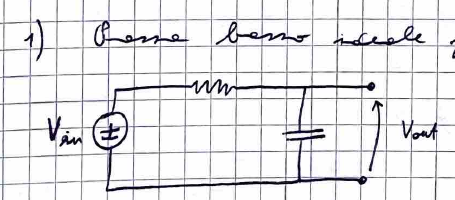
\includegraphics[width=0.65\linewidth]{elettrotecnica_figure/p31_1.png}
\end{center}
% Pagina originale 32
\pagina{32}{Filtri e autoinduzione}
2) Passa alto ideale passivo: resistore in serie e induttore in derivazione, uscita sull'induttore. Lascia passare $f>f_1$.
\[f\to0\Rightarrow V_{out}=0,\quad f\to\infty\Rightarrow V_{out}\ne0,\quad H(\omega)=\frac{V_{out}}{V_{in}}=\frac{j\omega L}{R+j\omega L}.\]
3) Passa banda: induttore e condensatore in serie, uscita sul resistore di chiusura. Lascia passare $f\simeq f_0$.
\[f\to0\ \wedge\ f\to\infty\Rightarrow V_{out}=0,\quad H(\omega)=\frac{V_{out}}{V_{in}}=\frac R{R+j\omega L-j/(\omega C)}.\]
4) Elimina banda: resistore in serie, condensatore e induttore in serie nel ramo di uscita. Lascia passare $f\ne f_0$.
\[f\to0\ \wedge\ f\to\infty\Rightarrow V_{out}\ne0,\quad H(\omega)=\frac{V_{out}}{V_{in}}=\frac{j(\omega L-1/(\omega C))}{R+j(\omega L-1/(\omega C))}.\]
\textbf{Autoinduzione.} Legge di Hopkinson:
\[\Phi_{g1}=\frac{N_1i_1}{\mathcal R_1},\quad\mathcal R_1=\frac\ell{\mu S},\quad\Phi_{\Sigma11}=N_1\Phi_{g1}=\frac{N_1^2i_1}{\mathcal R_1}.\]
\[v_{L1}=\frac{d\Phi_{\Sigma11}}{dt}=\frac{N_1^2}{\mathcal R_1}\frac{di_1}{dt}=L_1\frac{di_1}{dt},\quad L_1=\frac{d\Phi_{\Sigma11}}{di_1}=\frac{N_1^2}{\mathcal R_1},\quad\dot V_{L1}=j\omega L_1\dot I_1.\]

\begin{center}
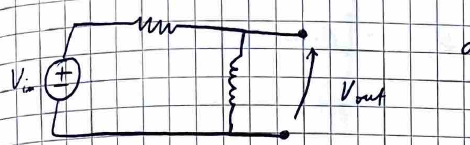
\includegraphics[width=0.40\linewidth]{elettrotecnica_figure/p32_1.png}
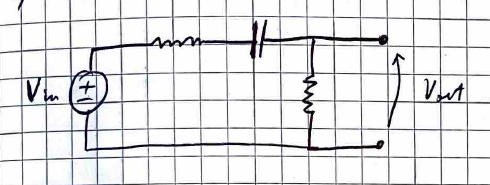
\includegraphics[width=0.40\linewidth]{elettrotecnica_figure/p32_2.png}
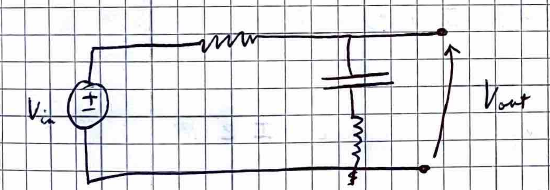
\includegraphics[width=0.40\linewidth]{elettrotecnica_figure/p32_3.png}
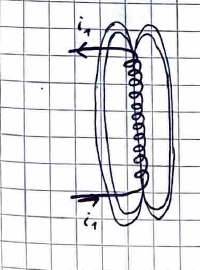
\includegraphics[width=0.40\linewidth]{elettrotecnica_figure/p32_4.png}
\end{center}
% Pagina originale 33
\pagina{33}{Mutua induzione e induttori accoppiati in serie}
\[\Phi_{g1}=\frac{N_1i_1}{\mathcal R_1},\quad\Phi_{\Sigma12}=N_2\Phi_{g1}=\frac{N_1N_2i_1}{\mathcal R_1},\]
\[M_{21}=\frac{d\Phi_{\Sigma12}}{di_1}=k_{12}\frac{N_1N_2}{\mathcal R_1}\quad[H],\]
\[v_{M21}=\frac{d\Phi_{\Sigma12}}{dt}=k_{12}\frac{N_1N_2}{\mathcal R_1}\frac{di_1}{dt}=M_{21}\frac{di_1}{dt},\quad\dot V_{M21}=j\omega M_{21}\dot I,\quad M_{ij}=M_{ji}.\]
\textbf{Collegamento induttori accoppiati: serie.}
\begin{align*}
V_{AB}&=V_{L1}+V_{L2}\pm V_{M21}\pm V_{M12}\\
&=L_1\frac{di}{dt}+L_2\frac{di}{dt}\pm M_{12}\frac{di}{dt}\pm M_{21}\frac{di}{dt}\\
&=(L_1+L_2\pm2M_{12})\frac{di}{dt}=L_{eq}\frac{di}{dt},\quad L_{eq}=L_1+L_2\pm2M_{12}.
\end{align*}
Nello schema dei quattro abbinamenti di morsetti: marcatura $\bullet$: $L_1+L_2+2M_{12}$; marcatura $*$: $L_1+L_2-2M_{12}$; marcatura $\times$: $L_1+L_2-2M_{12}$; marcatura $\triangle$: $L_1+L_2+2M_{12}$.

\begin{center}
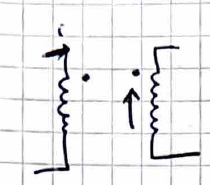
\includegraphics[width=0.40\linewidth]{elettrotecnica_figure/p33_1.png}
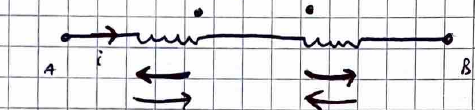
\includegraphics[width=0.40\linewidth]{elettrotecnica_figure/p33_2.png}
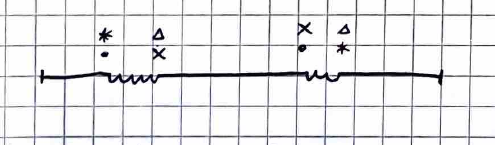
\includegraphics[width=0.40\linewidth]{elettrotecnica_figure/p33_3.png}
\end{center}
% Pagina originale 34
\pagina{34}{Induttori accoppiati in parallelo ed energia}
Due rami $R_1,L_1$ e $R_2,L_2$ in parallelo ai morsetti $A,B$, alimentati da $I_g$, con induttori accoppiati:
\[\bar Z_1=R_1+j\omega L_1,\quad\bar Z_2=R_2+j\omega L_2,\quad\bar Z_M=j\omega M.\]
\[\begin{cases}V_{AB}=\bar Z_1\dot I_1\pm\bar Z_M\dot I_2,\\V_{AB}=\bar Z_2\dot I_2\pm\bar Z_M\dot I_1.\end{cases}\]
\[\Delta=\begin{vmatrix}\bar Z_1&\pm\bar Z_M\\\pm\bar Z_M&\bar Z_2\end{vmatrix}=\bar Z_1\bar Z_2-\bar Z_M^2,\]
\[\Delta_{I_1}=\begin{vmatrix}V_{AB}&\pm\bar Z_M\\V_{AB}&\bar Z_2\end{vmatrix}=V_{AB}(\bar Z_2\mp\bar Z_M),\quad\Delta_{I_2}=\begin{vmatrix}\bar Z_1&V_{AB}\\\pm\bar Z_M&V_{AB}\end{vmatrix}=V_{AB}(\bar Z_1\mp\bar Z_M).\]
\[\dot I_1=\frac{V_{AB}(\bar Z_2\mp\bar Z_M)}{\bar Z_1\bar Z_2-\bar Z_M^2},\quad\dot I_2=\frac{V_{AB}(\bar Z_1\mp\bar Z_M)}{\bar Z_1\bar Z_2-\bar Z_M^2},\]
\[\dot I=\dot I_1+\dot I_2=\frac{V_{AB}(\bar Z_2+\bar Z_1\mp2\bar Z_M)}{\bar Z_1\bar Z_2-\bar Z_M^2},\quad\bar Z_{eq}=\frac{V_{AB}}{\dot I}\Rightarrow\dot I=\frac{V_{AB}}{\bar Z_{eq}},\]
\[\bar Z_{eq}=\frac{\bar Z_1\bar Z_2-\bar Z_M^2}{\bar Z_1+\bar Z_2\mp2\bar Z_M}.\]
Segno $-$: concordi; segno $+$: discordi.

\textbf{Energia accoppiamento mutuo.} Usiamo il PSE.
1) $i_1=0\to I_1$, $i_2=0$ ($di_2/dt=0$):
\[V'_{L1}=L_1\frac{di_1}{dt},\quad V'_{L2}=L_2\frac{di_2}{dt}=0,\quad V'_{M21}=M_{21}\frac{di_1}{dt},\quad V'_{M12}=M_{12}\frac{di_2}{dt}=0.\]

\begin{center}
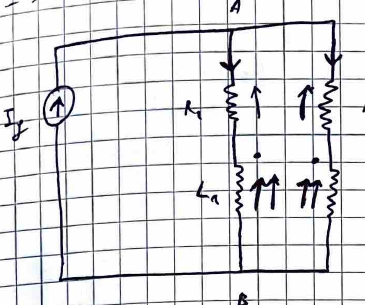
\includegraphics[width=0.65\linewidth]{elettrotecnica_figure/p34_1.png}
\end{center}
% Pagina originale 35
\pagina{35}{Energia e leggi di Kirchhoff magnetiche}
\[P'_1=i_1L_1\frac{di_1}{dt},\quad P'_2=M_{21}\frac{di_2}{dt}i_2=0,\]
\[W'_1=\int_0^tP'_1dt=\int_0^tL_1i_1\frac{di_1}{dt}dt=\int_0^{I_1}L_1i_1di_1=\frac12L_1I_1^2.\]
\emph{Nota: il termine $P'_2$ conserva l'indice e la derivata presenti nella fonte.}
2) $i_1=I_1$ ($di_1/dt=0$), $i_2=0\to I_2$:
\[V''_{L1}=L_1\frac{di_1}{dt}=0,\quad V''_{L2}=L_2\frac{di_2}{dt},\quad V''_{M21}=M_{21}\frac{di_1}{dt}=0,\quad V''_{M12}=M_{12}\frac{di_2}{dt},\]
\[P''_1=M_{12}\frac{di_2}{dt}I_1,\quad P''_2=L_2\frac{di_2}{dt}i_2,\]
\[W''_1=\int_0^tM_{12}\frac{di_2}{dt}I_1dt=\int_0^{I_2}M_{12}I_1di_2=M_{12}I_1I_2,\]
\[W''_2=\int_0^tL_2\frac{di_2}{dt}i_2dt=\int_0^{I_2}L_2i_2di_2=\frac12L_2I_2^2,\quad W=\frac12L_1I_1^2+\frac12L_2I_2^2+M_{12}I_1I_2.\]
Se parto con $i_2=0\to I_2$ mentre $i_1=0$ e poi pongo $i_1=0\to I_1$ mentre $i_2=I_2$, ottengo
\[W=\frac12L_1I_1^2+\frac12L_2I_2^2+M_{21}I_1I_2,\]
che deve essere per forza uguale, quindi $M_{12}=M_{21}$.

\textbf{Leggi di Kirchhoff magnetiche.} 1. Somma dei flussi in un nodo è nulla. 2. Somma delle tensioni magnetiche lungo un percorso chiuso (maglia) è uguale alla somma delle forze magnetomotrici presenti nel percorso.
% Pagina originale 36
\pagina{36}{Nuclei ferromagnetici e trasformatore}
\[L_1=\frac{N_1^2}{\mathcal R_{eq}},\quad\mathcal R=\frac\ell{\mu_0\mu_rS},\quad M_{12}=\alpha_{21}(1-\beta)\frac{N_1N_2}{\mathcal R_{eq1}},\]
\[M_{12}=k_{12}\sqrt{L_1L_2}=k_{12}\frac{N_1N_2}{\sqrt{\mathcal R_{eq1}\mathcal R_{eq2}}},\quad M_{12}=\alpha_{21}\frac{N_1N_2}{\mathcal R_{eq1}}\Rightarrow\frac{\alpha_{12}}{\mathcal R_{eq1}}=\frac{\alpha_{21}}{\mathcal R_{eq2}}.\]
\emph{Nota: indici conservati come nella fonte; accanto a $(1-\beta)$ un richiamo sembra indicare $\beta=0$.}
Se $\mathcal R_{eq1}=\mathcal R_{eq2}$, $\alpha_{12}=\alpha_{21}=k_{12}$.

\textbf{Trasformatore.} È un dispositivo elettromagnetico che sfrutta la mutua induzione per trasformare le tensioni ai due terminali d'ingresso in una tensione a due terminali d'uscita. Avvolgimento primario: $R_1,L_1$ con ingresso $V_{in}$ alimentato da $\dot E$; avvolgimento secondario: $R_2,L_2$, uscita $V_{out}$ sul carico $\bar Z_{CA}$.
\textbf{Impedenza d'ingresso:} $\bar Z_{in}=\dot E/\dot I$. Risolvo il sistema a due LKT per avvolgimenti ed ottengo
\[\bar Z_{in}=R_1+j\omega L_1+\frac{\omega^2M^2}{R_2+j\omega L_2+\bar Z_{CA}}.\]

\begin{center}
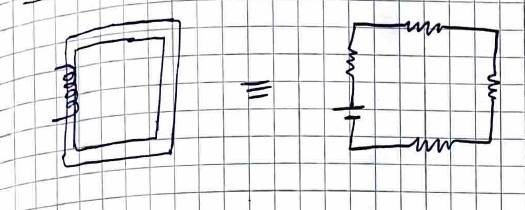
\includegraphics[width=0.40\linewidth]{elettrotecnica_figure/p36_1.png}
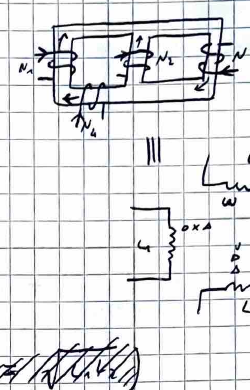
\includegraphics[width=0.40\linewidth]{elettrotecnica_figure/p36_2.png}
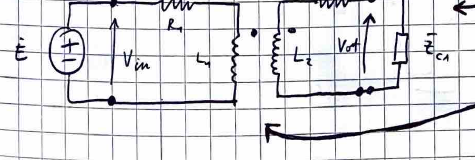
\includegraphics[width=0.40\linewidth]{elettrotecnica_figure/p36_3.png}
\end{center}
% Pagina originale 37
\pagina{37}{Trasformatore ideale e autotrasformatore}
Un trasformatore è ideale quando: gli avvolgimenti hanno reattanza elevata ($L_1,L_2\to\infty$); non vi sono perdite ($R_1=0\wedge R_2=0$); l'accoppiamento è perfetto ($k=1$).
\[\begin{cases}\dot V_1=j\omega L_1\dot I_1-j\omega M\dot I_2,\\\dot V_2=-j\omega L_2\dot I_2+j\omega M\dot I_1.\end{cases}\]
\[\dot I_1=\frac{\dot V_1+j\omega M\dot I_2}{j\omega L_1},\quad\dot V_2=-j\omega L_2\dot I_2+j\omega M\frac{\dot V_1+j\omega M\dot I_2}{j\omega L_1},\]
\[\dot V_2=-j\omega L_2\dot I_2+\frac{M\dot V_1}{L_1}+j\omega\frac{M^2}{L_1}\dot I_2.\]
Per $M=k\sqrt{L_1L_2}=\sqrt{L_1L_2}$:
\[\dot V_2=-j\omega L_2\dot I_2+\sqrt{\frac{L_2}{L_1}}\dot V_1+j\omega L_2\dot I_2=\sqrt{\frac{L_2}{L_1}}\dot V_1,\quad\sqrt{\frac{L_2}{L_1}}=\frac{N_2}{N_1}=n,\quad L=\frac{N^2}{\mathcal R_{eq}}.\]
\[\begin{array}{c|c|l}V_2>V_1&n>1&\text{elevatore}\\V_2=V_1&n=1&\text{isolamento}\\V_2<V_1&n<1&\text{riduttore}\end{array}\]
\[P_{in}=P_{out}\quad\text{(non ci sono perdite)},\quad\dot V_1\dot I_1=\dot V_2\dot I_2\Rightarrow\frac{\dot V_2}{\dot V_1}=\frac{\dot I_1}{\dot I_2}=n.\]
\[\bar Z_{in}=\frac{\dot V_1}{\dot I_1}=\frac{\dot V_1\dot I_2\dot V_2}{\dot I_1\dot I_2\dot V_2}=\frac{\dot V_2}{\dot I_2}\frac1n\frac1n=\bar Z_{out}\frac1{n^2}\Rightarrow\bar Z_{out}=n^2\bar Z_{in}\Rightarrow\frac{\bar Z_{out}}{\bar Z_{in}}=n^2.\]
\textbf{Autotrasformatore.} Nell'autotrasformatore il primario ed il secondario risiedono nello stesso avvolgimento.

\begin{center}
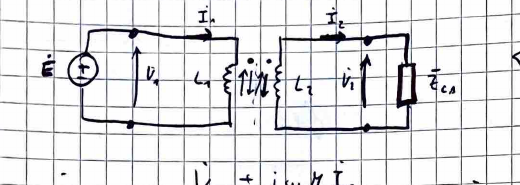
\includegraphics[width=0.65\linewidth]{elettrotecnica_figure/p37_1.png}
\end{center}
% Pagina originale 38
\pagina{38}{Trifase}
\[v_1=V_p\sin\omega t,\quad v_2=V_p\sin(\omega t\mp2\pi/3),\quad v_3=V_p\sin(\omega t\mp4\pi/3).\]
\begin{align*}
V_p\angle0^\circ+V_p\angle(-120^\circ)+V_p\angle120^\circ
&=V_p(1+\cos120^\circ-j\sin120^\circ+\cos120^\circ+j\sin120^\circ)\\
&=V_p(1+2(-1/2))=0.
\end{align*}
\[\dot V_{an}+\dot V_{bn}+\dot V_{cn}=0,\quad|\dot V_{an}|=|\dot V_{bn}|=|\dot V_{cn}|=V_p\quad\text{tensione di fase}.\]
\[\dot V_{ab}=\dot V_{an}+\dot V_{nb}=\dot V_{an}-\dot V_{bn}=V_p\left(\frac32+j\frac{\sqrt3}2\right)=\sqrt3V_p\angle30^\circ,\quad V_L=\sqrt3V_p.\]
Tensione di fase: $220\,V$; tensione di linea: $380\,V$ (valori conservati dall'originale).
\begin{center}\begin{tikzpicture}[>=stealth,scale=.9]
\draw[->] (0,0)--(2.6,0) node[right] {$\dot V_{an}$};\draw[->] (0,0)--(-1.3,-2.25) node[below] {$\dot V_{bn}$};\draw[->] (0,0)--(-1.3,2.25) node[above] {$\dot V_{cn}$};
\draw[->,thick] (0,0)--(3.9,2.25) node[right] {$\dot V_{ab}$};\draw[->,thick] (0,0)--(0,-4.5) node[below] {$\dot V_{bc}$};\draw[->,thick] (0,0)--(-3.9,2.25) node[left] {$\dot V_{ca}$};\draw[dashed] (2.6,0)--(3.9,2.25);\draw[dashed] (-1.3,-2.25)--(0,-4.5);\draw[dashed] (-1.3,2.25)--(-3.9,2.25);\draw (0.8,0) arc(0:30:0.8) node[midway,right] {$30^\circ$};\node at (1,-1) {di fase};\node at (2,-3) {di linea};
\end{tikzpicture}\end{center}
\end{document}
